% !TeX root = chapter-6-7-8.tex

\selectlanguage{hebrew}

\section*{המלצות}

\addcontentsline{cot}{chapter}{המלצות}

\begin{itemize}
\item
אי-אפשר להכין טבלה של עליות וירידות עד שלא מחשבים את תחום ההגדרה 
\textbf{וגם}
כל נקודות הקיצון של הפנוקציה, כי רק ביניהם אפשר לסמוך על זה שאין שינוי בכיוון הפונקציה.


\item
אני אוהב להשתמש בתנועות ידיים כדי "לראות שיפועים" ולקבוע אם פונקציה עולה או יורדת, וכן אם נקודות קיצון היא מקסימום או מינימים. אני מזיז כף יד שטוחה לאורך הפונקציה מערכים שליליים לחיוביים על ציר ה-%
$x$.
אם כיוון היד למטה הפונקציה יורדת, ואם הכיוון למעלה הפונקציה עולה. אם היד עוברת מכיוון למטה לכיוון למעלה, השיפוע )הנגזרת( עולה, כך שהנגזרת השנייה היא חיובית ונקודת הקיצון היא מינימים. שינוי הפוך בכיוון היד מראה שקיים מקסימום.

\item
אני מציע להתרחק מהמחשבון עד כמה שאפשר ולחשב עם סימנים אלגבריים. הסיבה היא שאי-אפשר למצוא בקלות שגיאות הנגרמות על ידי טעויות בקלדה על המחשבון, אבל אפשר לעבור שוב ושוב על חישוב אלגבראי כדי לוודא את נכונותו. 

\item
אל תקצרו בחישובים. לעתים קרובות שגיתי כי השמטתי סימן מינוס בטעות. לוקח מעט זמן לרשום שורה נוספת, לעומת הזמן הדרוש לחפש שגיאה בחישוב מקוצר.

\item
בבעיות עם פונקציות טריגונומטריות, ציירו תרשים של מעגל היחידה וסמנו 
\begin{center}
\selectlanguage{english}
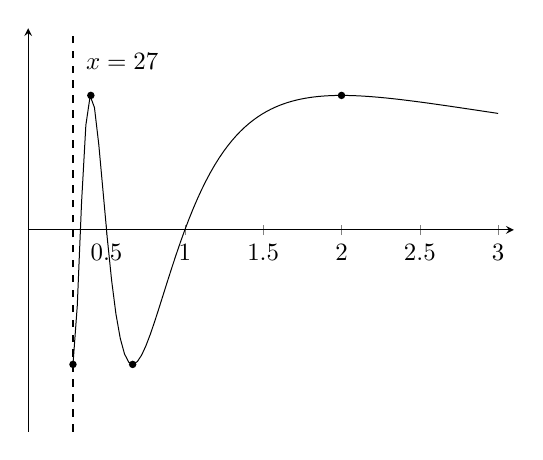
\begin{tikzpicture}[scale=.9]
\begin{axis}[
    trig format plots=rad,
    axis lines=center,
    xmin = 0,
    xmax = 3.1,
    ymin = -1.5,
    ymax = 1.5,
    ymajorticks=false,
]
\addplot [
    domain=.286:3,
    samples=100, 
]
{sin(rad 3.14159/rad x)};
\draw[dashed,thick] (axis cs:.286,-1.5) -- (axis cs:.286,1.5);
\fill (axis cs:.286,-1) circle(1.5pt);
\fill (axis cs:.667,-1) circle(1.5pt);
\fill (axis cs:.4,1) circle(1.5pt);
\fill (axis cs:2,1) circle(1.5pt);
\node at (axis cs:.6,1.25) {$x=\disfrac{2}{7}$};
\end{axis}
\end{tikzpicture}
\end{center}
עליו את תחום ההגדרה. התרשים יעזור בקביעת סימני הפונקציות ובערכי הפונקציות כאשר מוסיפים או מחסירים כפולות רציונליות של 
$\pi$.

\item 
שימו לב להבדל בין שטח לאיטגרל. ההבדל בין שטח לאיטגרל. למשל, אם מבקשים את האיטגרל של סינוס מאפס עד 
$2\pi$,
התשובה היא אפס:
\[
\int_0^{2\pi} \sin x\, dx =-\left.\cos x\right|_0^{2\pi}= -(1-1)=0\,.
\]

\vspace{-4ex}

אבל אם מבקשים את השטח התחום על ידי הפונקציה וציר ה-%
$x$
התשובה היא:
\[
\int_0^{\pi} \sin x\, dx + \int_{\pi}^{2\pi} -\sin x\, dx = -\left.\cos x\right|_0^{\pi} \left.+\cos x\right|_{\pi}^{2\pi}= -(-1-(1))+(1-(-1))=4\,.
\]

\np

\begin{center}
\selectlanguage{english}
\begin{tikzpicture}[scale=.9]
\begin{axis}[
    trig format plots=rad,
    axis lines=center,
    xmin = 0,
    xmax = 7,
    ymin = -1.1,
    ymax = 1.1,
    xtick={0,3.14,6.28},
    xticklabels={$0$, $\pi$, $2\pi$},
    xticklabel style={anchor=south west},
]
\addplot [
    domain=0:6.28,
    samples=60, 
]
{sin(x)};
\end{axis}
\end{tikzpicture}
\end{center}

\item
איטגרל של פונקציה אי-זוגית בתחום סימטרי סביב ציר ה-%
$y$
הוא אפס, ואינטגרל של פונקציה זוגית בתחום סימטרי הוא פי שניים האינטגרל של התחום החיובי בלבד.



\end{itemize}

\selectlanguage{english}

